\section{Architektura systemu Salomon}
\subsection{Architektura}
\frame{
	\frametitle{Architektura}
	
	\begin{columns}[t]
		\begin{column}{0.5\textwidth}
			\begin{center}
			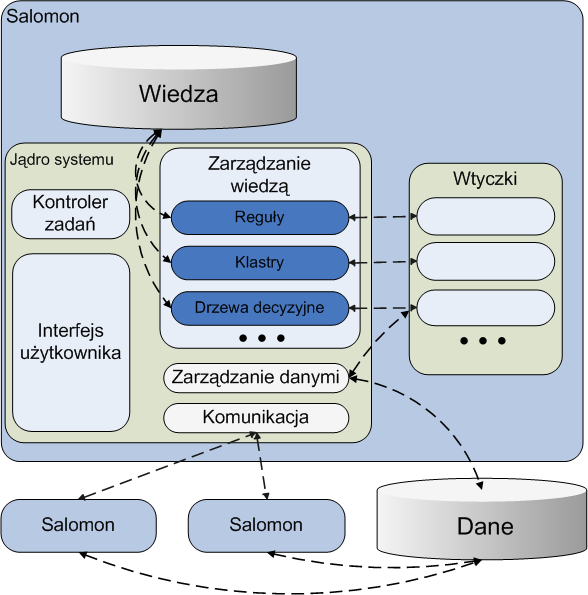
\includegraphics[width=\textwidth]{img/architecture.png}
		\end{center}
		\end{column}
	
		\begin{column}{0.5\textwidth}
		\begin{elements}
		\begin{itemize}
    		\item Instancje
    		\item J�dro
    		\item Interfejs u�ytkownika
    		\item Modu� zarz�dzaj�cy wiedz�
    		\item Modu� zarz�dzaj�cy danymi
    		\item Modu� komunikacyjny
    		\item Wtyczki
    		\item Dane
    		\item Wiedza
    		\item Kontroler zada�
    \end{itemize}
    \end{elements}
    \end{column}
	\end{columns}
}

\subsection{Warstwy}
\frame{
	\frametitle{Warstwy}
	\begin{itemize}
    	\item Komunikacja z zewn�trznymi �r�d�ami danych
    	\item Komunikacja mi�dzy r�nymi instancjami Salomona
    	\item Komunikacja z wtyczkami
    	\item Interfejs u�ytkownika
    \end{itemize}
}
